\documentclass[class=article, float=false, crop=false]{standalone}
\usepackage[subpreambles=true]{standalone}

\input{preamble}

\graphicspath{{figures/images/}}

% \begin{cbunit}

\begin{document}

\section{Nematic order close to the jamming transition}
\label{sec:jamming}

We have in the study of Nascimento \textit{et al.} \cite{nascimento2017density} that the nematic order of the static packing of spheroids tends to 1 when increasing its density. Therefore, their densest packing possible is a crystal array, as in \cite{donev2004unusually}.\\

However, it has been reported that no orientational order is present at jamming \cite{donev2004improving,PRL94.198001}. In order to investigate this, we will here report on shearing simulations conducted on packings of soft-core frictionless spheroids with harmonic repulsive interaction. In these simulations, the control parameters relevant to the jamming transition are the packing fraction $\phi$ and the shear rate $\dot{\gamma}$.

\subsection{Jamming as a critical phenomenon}

\subsubsection{Critical behaviour}

In the vicinity of the jamming transition, we have that the shear viscosity $\eta \equiv \sigma/\dot{\gamma}$ -- with $\sigma$ the shear stress and $\dot{\gamma}$ the shear strain rate, -- or equivalently the pressure viscosity $\eta_p \equiv p/\dot{\gamma}$ -- with $p$ the pressure, -- and a correlation length scale $\xi$ diverge as
\begin{equation}
% \boxed{
\begin{aligned}
\eta,\eta_p \isEquivTo{\phi\rightarrow\phi_J} \left(\phi_J - \phi\right)^{-\beta}\\
\xi \isEquivTo{\phi\rightarrow\phi_J} \left(\phi_J - \phi\right)^{-\nu}
\end{aligned}
% }
\label{critical_exponents}
\end{equation}
for soft-core particles in the limit $\dot{\gamma}\rightarrow0$ \cite{PRL99.178001,PRE83.030302} and for hard-core particles \cite{PRL109.108001}. This power-law divergence of the transport coefficient and of a correlation length scale are reminiscent of the behaviour near a critical point \cite{PRE83.030302,plischke1994equilibrium,PRE83.030303} of a second-order continuous phase transition.

\subsubsection{Scaling analysis}

Because the pressure viscosity varies on a larger interval than the nematic order parameter, we will perform our scaling analysis on the former. We detail here how what they consist of.\\

% First of all, we always assume that our system is in the thermodynamic limit $N\rightarrow+\infty \Leftrightarrow 1/L \rightarrow 0$, where $L$ is the characteristic length and then neglect any finite-size effect arising from the finite number of particles $N$ composing the system.\\

Renormalisation group theory suggests that for an infinite system close to the jamming point, \textit{i.e.} $(\phi_J-\phi=\delta\phi\rightarrow0,\dot{\gamma}\rightarrow0)$, there exists $y_{\delta\phi}$ and $y_{\dot{\gamma}}$ such that the correlation length transforms under a change of length scale with a factor $l$ as
\begin{align*}
\xi(\delta\phi,\dot{\gamma}) = l\xi(\delta\phi l^{y_{\delta\phi}},\dot{\gamma}l^{y_{\dot{\gamma}}})
\end{align*}
which, when choosing $l$ such that $\delta\phi l^{y_{\delta\phi}}=b \Leftrightarrow l=\left(\frac{\delta\phi}{b}\right)^{-1/y_{\delta\phi}} \ge 1$, gives
\begin{align*}
\xi(\delta\phi,\dot{\gamma}) = \left(\frac{\delta\phi}{b}\right)^{-1/y_{\delta\phi}} \xi\left(b,\dot{\gamma}\left(\frac{\delta\phi}{b}\right)^{-y_{\dot{\gamma}}/y_{\delta\phi}}\right) \isEquivTo{\delta\phi\rightarrow0} (\delta\phi)^{-1/y_{\delta\phi}}
\end{align*}
where we recognise $\nu=1/y_{\delta\phi} > 0$ according to equation \ref{critical_exponents}.\\

We will assume that variables which vanish at jamming are somehow linked to the free energy density of the system. Therefore, in accordance with renormalisation group theory, we here suggest the following assumption on the scaling of a vanishing variable $\mathcal{O}$ close to the jamming point for a change of length scale with a factor $l$ 
\begin{equation}
\mathcal{O}(\delta\phi,\dot{\gamma}) \sim l^{-y_{\mathcal{O}}/\nu} g_{\mathcal{O}}(\delta\phi l^{1/\nu},\dot{\gamma}l^z)
\label{scaling_assumption_general}
\end{equation}
where we can choose $\delta\phi l^{1/\nu}=b \Leftrightarrow l=\left(\frac{\delta\phi}{b}\right)^{-\nu} \ge 1$ and deduce
\begin{align*}
\mathcal{O}(\delta\phi,\dot{\gamma}) \sim \left(\frac{\delta\phi}{b}\right)^{y_{\mathcal{O}}} g_{\mathcal{O}}\left(b,\dot{\gamma}\left(\frac{\delta\phi}{b}\right)^{-\nu z}\right)
\end{align*}
where we take the $\delta\phi\rightarrow0$ limit, which gives
\begin{equation}
\mathcal{O}(\delta\phi,\dot{\gamma}) \isEquivTo{\delta\phi\rightarrow0} (\delta\phi)^{y_{\mathcal{O}}}
\end{equation}
with $y_{\mathcal{O}} > 0$ thus being the critical exponent associated to the vanishing of the variable $\mathcal{O}$ at jamming.\\

We introduce the function $\tilde{g}_p$ such that equation \ref{scaling_assumption_general} applied to the pressure $p$ can be written
\begin{align*}
p(\delta\phi,\dot{\gamma}) \sim \dot{\gamma} l^z l^{-y_p/\nu} \tilde{g}_p(\delta\phi l^{1/\nu},\dot{\gamma}l^z)
\end{align*}
and then choose $l$ such that $\delta\phi l^{1/\nu} = b \Leftrightarrow l = \left(\frac{\delta\phi}{b}\right)^{-\nu} \ge 1$, which leads to
\begin{align*}
p(\delta\phi,\dot{\gamma}) \sim \dot{\gamma} \left(\frac{\delta\phi}{b}\right)^{-(\nu z-y)} \tilde{g}_p\left(b,\dot{\gamma}\left(\frac{\delta\phi}{b}\right)^{-\nu z}\right)
\end{align*}
and therefore
\begin{equation}
\eta_p(\delta\phi,\dot{\gamma}) \equiv p(\delta\phi,\dot{\gamma})/\dot{\gamma} \isEquivTo{\delta\phi\rightarrow0} (\delta\phi)^{-(\nu z-y)}
\end{equation}
where we recognise $\beta=\nu z-y$ according to equation \ref{critical_exponents}.\\

We now choose $l$ such that $\dot{\gamma}l^z = b \Leftrightarrow l = \left(\frac{\dot{\gamma}}{b}\right)^{-1/z} \ge 1$, which put in equation \ref{scaling_assumption_general} for $p$ leads to
\begin{align*}
p(\delta\phi,\dot{\gamma}) \sim \dot{\gamma}^{y_p/\nu z} g_p\left(\delta\phi \left(\frac{\dot{\gamma}}{b}\right)^{-1/\nu z},b\right)
\end{align*}
and finally introduce the function $g_p^{(\text{fit})}$ in order to ignore the constant $b$ in this last equation, which becomes
\begin{equation}
p(\delta\phi,\dot{\gamma}) \sim \dot{\gamma}^{y_p/\nu z} g_p^{(\text{fit})}(\delta\phi\dot{\gamma}^{-1/\nu z})
\label{fitting_function_form}
\end{equation}
and in which we will denote $q_p\equiv y_p/\nu z$ and $h_p\equiv -1/\nu z$, thus leading to $\beta=(q_p-1)/h_p$, in addition to $Y_p \equiv p(\delta\phi,\dot{\gamma})\dot{\gamma}^{-q_p}$ and $X_p \equiv \delta\phi\dot{\gamma}^{h_p}$.\\

% A graphical method to determine the values of $\phi_J$ and $q_p$, based on the study of equation \ref{fitting_function_form}, is described in \cite{PRE83.030302}, we will however use a different method that allows us to determine these parameters and $h_p$, and therefore find the critical exponent $\beta$.\\

Equation \ref{fitting_function_form} suggests that it is possible to collapse the data from simulations at different packing fractions and shear strain rates on a single curve in the ($X_{p}$,$Y_{p}$) plane. To perform this fitting, we choose arbitrarily the expression of $g_{\mathcal{O}}^{(\text{fit})}$
\begin{align*}
g_{p}^{(\text{fit})}:X_{p}\mapsto\exp\left(\sum_{i=0}^5a_{p,i}X_{p}^i\right)
\end{align*}
and use the Levenberg-Marquardt algorithm \cite{marquardt1963algorithm,press2015numerical} with $\phi_J$, $z_c$, $q_{p}$, $h_{p}$ and $a_{p,0}$ through $a_{p,5}$ as free parameters.% to the corresponding variable fitting. The goal of this algorithm is to minimise the deviation of the experimental data from the fitted curve with respect to the standard deviation for each ``experimental'' point.

\subsubsection{Soft- to hard-core mapping}

Shearing simulations are more easily conducted with soft-core particles. However, we are interested in the behaviour of hard-core packings near jamming, we thus have to remove the effect of the particles interpenetration in our data.\\

We can find in \cite{PRL109.108001} a method to map soft-core particles at a given packing fraction $\phi$ and shear strain rate $\dot{\gamma}$ to equivalent hard-core particles at a lesser packing fraction $\phi_{\text{eff}}$ such as
\begin{equation}
\begin{aligned}
\eta^s_p(\phi,\dot{\gamma}) &= \eta^s_p(\phi_{\text{eff}},\dot{\gamma}\rightarrow0)\\
\eta^h_p(\phi_{\text{eff}}) &\equiv \eta^s_p(\phi_{\text{eff}},\dot{\gamma}\rightarrow0) \isEquivTo{\phi_{\text{eff}}\rightarrow\phi_J} \left(\phi_J - \phi_{\text{eff}}\right)^{-\beta}
\label{phieff}
\end{aligned}
\end{equation}
according to equation \ref{critical_exponents}.\\

This mapping is done by assuming that $\phi_{\text{eff}}$ is determined by the extent of particle overlaps, measured by the average energy per particle $E(\phi,\dot{\gamma})$. Authors of \cite{PRL109.108001} then proposed the following relation
\begin{equation}
\phi_{\text{eff}}(\phi,\dot{\gamma}) = \phi - h(E(\phi,\dot{\gamma}))
\label{phieff_}
\end{equation}
where $h$ can be determined asymptotically close to $\phi_J$. Indeed, further considerations on the jamming transition gives us the following expression

% We can first notice that there is no distinction between soft-core and hard-core particles in a system where the particles do not overlap. In such a system, the average energy per particle equals to $0$, therefore we must have
% \begin{equation}
% h(0)=0
% \end{equation}

% In a jammed system -- \textit{i.e.}, $\phi\ge\phi_J$ -- of soft-core particles, particles have no choice but to overlap leading to $p > 0$ even as $\dot{\gamma} \rightarrow 0$, and then $\eta_p^s(\phi\ge\phi_J,\dot{\gamma}\rightarrow0)\rightarrow+\infty$. In consequence, according to equation \ref{phieff}, we must have $\eta^h_p(\phi_{\text{eff}})\rightarrow+\infty$, which is only achieved for a system of hard-core particles at $\phi_{\text{eff}}=\phi_J$, therefore
% \begin{equation}
% \begin{aligned}
% \phi_{\text{eff}}(\phi\ge\phi_J,\dot{\gamma}\rightarrow0) = \phi_J\\
% \end{aligned}
% \label{phiefflimit}
% \end{equation}

% From equations \ref{phieff_} and \ref{phiefflimit}, we have that
% \begin{align*}
% \phi_{\text{eff}}(\phi\ge\phi_J,\dot{\gamma}\rightarrow0) = \phi - h(E(\phi,\dot{\gamma}\rightarrow0)) = \phi_J \Rightarrow h(E(\phi,\dot{\gamma}\rightarrow0)) = \phi-\phi_J
% \end{align*}
% and, since $E(\phi,\dot{\gamma}\rightarrow0)$ vanishes algebraically close to $\phi_J$, we can write
% \begin{align*}
% E(\phi,\dot{\gamma}\rightarrow0) \isEquivTo{\phi\rightarrow\phi_J} (\phi-\phi_J)^{y_E} &\Leftrightarrow E(\phi,\dot{\gamma}\rightarrow0)^{1/y_E} \isEquivTo{\phi\rightarrow\phi_J} \phi-\phi_J\\
% &\Rightarrow E(\phi,\dot{\gamma}\rightarrow0)^{1/y_E} \isEquivTo{\phi\rightarrow\phi_J} h(E(\phi,\dot{\gamma}\rightarrow0))\\
% &\Rightarrow X^{1/y_E} \isEquivTo{X\rightarrow0} h(X)
% \end{align*}
% where the latter equivalence can be applied to $E(\phi,\dot{\gamma})$ in the vicinity of $\phi_J$, therefore
\begin{equation}
\phi_{\text{eff}}(\phi,\dot{\gamma})\operatorname*{~=~}_{\phi\rightarrow\phi_J}\phi-cE(\phi,\dot{\gamma})^{1/y_E}
\label{phieff_soft2hard}
\end{equation}
with $c$ a constant.\\

In our model of harmonic elastic interactions, the pressure and the energy scale as $E \sim p^2$. Therefore, we have that $y_E$ satifies the following relation
\begin{equation}
y_E = 2y_p \Leftrightarrow y_E = -2q_p/h_p
\end{equation}
Therefore, considering that $q_p$ and $h_p$ have been determined with our scaling method, $c$ remains the only unknown variable in equation \ref{phieff_soft2hard}.\\
% We then have a quick way to check the efficiency of this method.\\

Equations \ref{phieff} and \ref{phieff_soft2hard} can be rewritten as
\begin{equation}
\eta_p^s(\phi,\dot{\gamma}) = A\left(\phi_J-\phi +cE(\phi,\dot{\gamma})^{-h_p/2q_p}\right)^{-\beta}
\label{phieff_soft2hard_check}
\end{equation}
where $A$ is an additional parameter which can be determined if we take two points $\eta_{p,1} \equiv \eta_p(\phi_1,\dot{\gamma}_1)$ and $\eta_{p,2} \equiv \eta_p(\phi_2,\dot{\gamma}_2)$, whose corresponding energies are $E_1 \equiv E(\phi_1,\dot{\gamma}_1)$ and $E_2 \equiv E(\phi_2,\dot{\gamma}_2)$, which we hypothesise satisfy equation \ref{phieff_soft2hard_check}. We can then isolate $c$ in equation \ref{phieff_soft2hard_check}, giving
\begin{align*}
c = E(\phi,\dot{\gamma})^{h_p/2q_p}\left(A^{1/\beta}\eta_p(\phi,\dot{\gamma})^{-1/\beta}-\phi_J+\phi\right)
\end{align*}
which has to be satisfied by the two aforementioned points, therefore
\begin{align*}
&E_1^{h_p/2q_p}\left(A^{1/\beta}\eta_{p,1}^{-1/\beta}-\phi_J+\phi_1\right) = E_2^{h_p/2q_p}\left(A^{1/\beta}\eta_{p,2}^{-1/\beta}-\phi_J+\phi_2\right)\\
\Leftrightarrow &A=\left(\left(\eta_{p,1}^{-1/\beta}E_1^{h_p/2q_p} - \eta_{p,2}^{-1/\beta}E_2^{h_p/2q_p}\right)^{-1}\left(E_1^{h_p/2q_p}(\phi_J-\phi_1) + E_2^{h_p/2q_p}(\phi_2-\phi_J)\right)\right)^{\beta}
\end{align*}
which can be re-injected in the expression of $c$ evaluated in either point.\\

% , therefore
% \begin{align*}
% &E_1^{h_p/2q_p}\left(A^{1/\beta}\eta_{p,1}^{-1/\beta}-\phi_J+\phi_1\right) = E_2^{h_p/2q_p}\left(A^{1/\beta}\eta_{p,2}^{-1/\beta}-\phi_J+\phi_2\right)\\
% \Leftrightarrow &A=\left(\left(\eta_{p,1}^{-1/\beta}E_1^{h_p/2q_p} - \eta_{p,2}^{-1/\beta}E_2^{h_p/2q_p}\right)^{-1}\left(E_1^{h_p/2q_p}(\phi_J-\phi_1) + E_2^{h_p/2q_p}(\phi_2-\phi_J)\right)\right)^{\beta}
% \end{align*}
% which can be re-injected in the expression of $c$ evaluated in either point.\\

This method enables us to do two things:
\begin{itemize}
\item Verify that the data for an other variable than the pressure is consistent with the latter. Indeed, if everything is consistent, we will see that the curves for different shear rates will collapse on a single curve.
\item Find the critical exponent associated to the vanishing of an other variable than the pressure with a simple linear regression rather than with the scaling analysis we have described.
\end{itemize}

% Another, more time-consuming, solution is of course to apply the Levenberg-Marquardt algorithm (part \ref{levenberg_marquadt}) on equation \ref{phieff_soft2hard_check} with $A$ and $c$ as free parameters.

\subsection{Nematic order}

We present here our results on the nematic order parameter $S$ in shearing simulations of spheroids in Figure \ref{Sphi_sheared}.

\begin{figure}[h!]
\centering
    \hfill
    \begin{subfigure}[t]{0.49\textwidth}
        \centering
        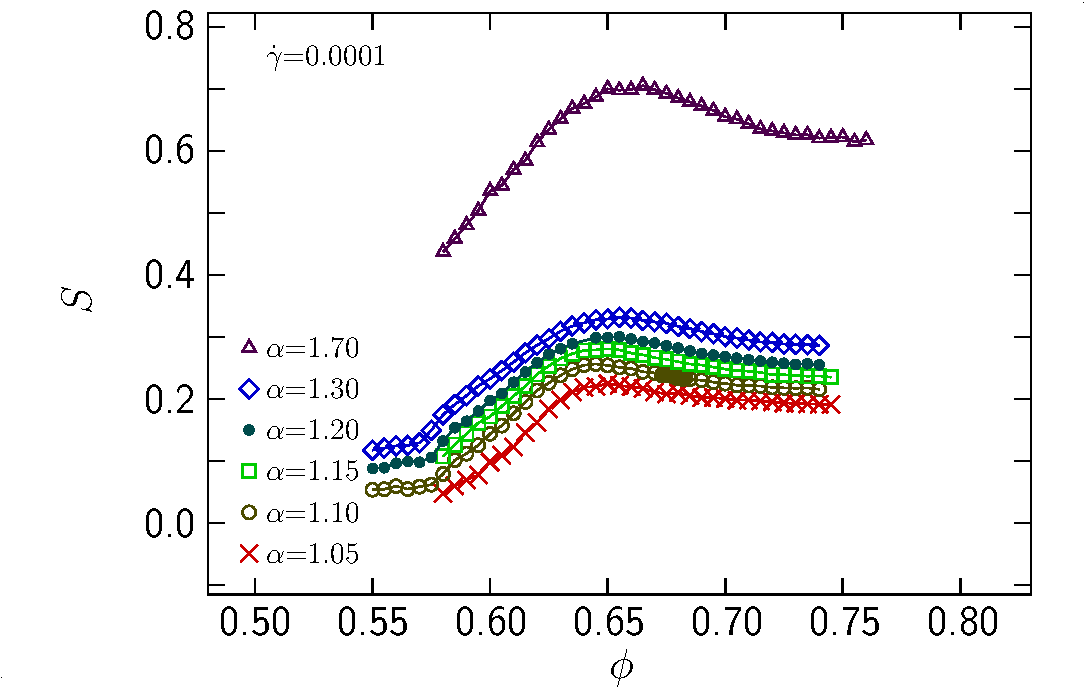
\includegraphics[width=\textwidth]{figures/figs/S_phi_el}
        \caption{Different aspect ratio and same shear rate.}
    \end{subfigure}
    \hfill
    \begin{subfigure}[t]{0.49\textwidth}
        \centering
        \includegraphics[width=\textwidth]{figures/figs/S2_phi_1024_KDk500_Ml100_EL170}
        \caption{Same aspect ration and different shear rate.}
    \end{subfigure}
    \hfill
\caption{Nematic order parameter $S$ as a function of the packing fraction $\phi$.}
\label{Sphi_sheared}
\end{figure}

We first observe that we always have a strictly positive $S$, \textit{i.e.} the system can never be described as an isotropic phase. Contrarily to the static packings we first studied in this essay, the isotropy of space is here broken by the shearing, such a result was then to be expected. Indeed, shear-alignment of anisotropic particles have already been reported. \cite{borzsonyi2012orientational} However, data at very low packing fractions where particles seldom come into contact, and thus are very little influenced by the shearing, could give a negligible nematic order parameter. In addition, we have regions of $\phi$ where $S$ is lesser than $S_{NI,\text{th.}}$, which is the minimum $S$ theoretically obtained for static packings. This also suggests that the origin of the orientational ordering in our sheared packings is different from its origin in static packings.\\

There is a first domain of packing fractions where $S$ is an increasing function of the packing fraction at fixed aspect ratio and where it does not depend on the shear rate, hence suggesting that this behaviour is linked to static -- rather than dynamic -- properties of the packings. It can be explained by the depletion of available orientation configurations with increasing packing fraction: the particles tend to align to decrease the excluded volume effect as we have seen before. This is consistent with $S$ being an increasing function of the aspect ratio at fixed packing fraction since the effects of excluded volumes increase with increasing aspect ratio.\\

We then have that $S$ reaches a maximum for a particular packing fraction before decreasing near the jamming density. This is the part we are interested in.\\

We apply the soft- to hard-core mapping technique we have presented to the nematic order parameter $S$. We see that data for different shear rates collapse on a single curve, hence showing that the data for $S$ is consistent with the data for $p$. We can then proceed to the linear regression in order to determine if, in the vicinity of the jamming transition, $S$ decreases algebraically with the distance to the jamming packing fraction as we would expect near a critical point. Results are presented in Figure \ref{scaling_S}.\\

\begin{figure}[h!]
\centering
\includegraphics[width=0.7\textwidth]{figures/figs/S2_scale_1024_KDk500_Ml100_EL170_2.pdf}
\caption{Nematic order parameter $S$ as a function of the effective packing fraction $\phi_{\text{eff}}$.}
\label{scaling_S}
\end{figure}

Our data then shows evidence for a critical vanishing of the nematic order parameter $S$ at the jamming transition which is consistent with the vanishing of the pressure. Despite the low error on the critical exponent, we still need more data closer to the jamming density to give a quantitative result.

% \input{references/biblio}

\end{document}

% \end{cbunit}